% Options for packages loaded elsewhere
\PassOptionsToPackage{unicode}{hyperref}
\PassOptionsToPackage{hyphens}{url}
%
\documentclass[
]{article}
\usepackage{amsmath,amssymb}
\usepackage{lmodern}
\usepackage{iftex}
\ifPDFTeX
  \usepackage[T1]{fontenc}
  \usepackage[utf8]{inputenc}
  \usepackage{textcomp} % provide euro and other symbols
\else % if luatex or xetex
  \usepackage{unicode-math}
  \defaultfontfeatures{Scale=MatchLowercase}
  \defaultfontfeatures[\rmfamily]{Ligatures=TeX,Scale=1}
\fi
% Use upquote if available, for straight quotes in verbatim environments
\IfFileExists{upquote.sty}{\usepackage{upquote}}{}
\IfFileExists{microtype.sty}{% use microtype if available
  \usepackage[]{microtype}
  \UseMicrotypeSet[protrusion]{basicmath} % disable protrusion for tt fonts
}{}
\makeatletter
\@ifundefined{KOMAClassName}{% if non-KOMA class
  \IfFileExists{parskip.sty}{%
    \usepackage{parskip}
  }{% else
    \setlength{\parindent}{0pt}
    \setlength{\parskip}{6pt plus 2pt minus 1pt}}
}{% if KOMA class
  \KOMAoptions{parskip=half}}
\makeatother
\usepackage{xcolor}
\IfFileExists{xurl.sty}{\usepackage{xurl}}{} % add URL line breaks if available
\IfFileExists{bookmark.sty}{\usepackage{bookmark}}{\usepackage{hyperref}}
\hypersetup{
  pdftitle={My Awesome Catchy Title!},
  pdflang={nl},
  hidelinks,
  pdfcreator={LaTeX via pandoc}}
\urlstyle{same} % disable monospaced font for URLs
\usepackage[margin=1in]{geometry}
\usepackage{longtable,booktabs,array}
\usepackage{calc} % for calculating minipage widths
% Correct order of tables after \paragraph or \subparagraph
\usepackage{etoolbox}
\makeatletter
\patchcmd\longtable{\par}{\if@noskipsec\mbox{}\fi\par}{}{}
\makeatother
% Allow footnotes in longtable head/foot
\IfFileExists{footnotehyper.sty}{\usepackage{footnotehyper}}{\usepackage{footnote}}
\makesavenoteenv{longtable}
\usepackage{graphicx}
\makeatletter
\def\maxwidth{\ifdim\Gin@nat@width>\linewidth\linewidth\else\Gin@nat@width\fi}
\def\maxheight{\ifdim\Gin@nat@height>\textheight\textheight\else\Gin@nat@height\fi}
\makeatother
% Scale images if necessary, so that they will not overflow the page
% margins by default, and it is still possible to overwrite the defaults
% using explicit options in \includegraphics[width, height, ...]{}
\setkeys{Gin}{width=\maxwidth,height=\maxheight,keepaspectratio}
% Set default figure placement to htbp
\makeatletter
\def\fps@figure{htbp}
\makeatother
\setlength{\emergencystretch}{3em} % prevent overfull lines
\providecommand{\tightlist}{%
  \setlength{\itemsep}{0pt}\setlength{\parskip}{0pt}}
\setcounter{secnumdepth}{5}
\newlength{\cslhangindent}
\setlength{\cslhangindent}{1.5em}
\newlength{\csllabelwidth}
\setlength{\csllabelwidth}{3em}
\newlength{\cslentryspacingunit} % times entry-spacing
\setlength{\cslentryspacingunit}{\parskip}
\newenvironment{CSLReferences}[2] % #1 hanging-ident, #2 entry spacing
 {% don't indent paragraphs
  \setlength{\parindent}{0pt}
  % turn on hanging indent if param 1 is 1
  \ifodd #1
  \let\oldpar\par
  \def\par{\hangindent=\cslhangindent\oldpar}
  \fi
  % set entry spacing
  \setlength{\parskip}{#2\cslentryspacingunit}
 }%
 {}
\usepackage{calc}
\newcommand{\CSLBlock}[1]{#1\hfill\break}
\newcommand{\CSLLeftMargin}[1]{\parbox[t]{\csllabelwidth}{#1}}
\newcommand{\CSLRightInline}[1]{\parbox[t]{\linewidth - \csllabelwidth}{#1}\break}
\newcommand{\CSLIndent}[1]{\hspace{\cslhangindent}#1}
\ifLuaTeX
\usepackage[bidi=basic]{babel}
\else
\usepackage[bidi=default]{babel}
\fi
\babelprovide[main,import]{dutch}
% get rid of language-specific shorthands (see #6817):
\let\LanguageShortHands\languageshorthands
\def\languageshorthands#1{}
\usepackage{setspace}
\doublespacing
\usepackage{float}
\let\origfigure\figure
\let\endorigfigure\endfigure
\renewenvironment{figure}[1][2] {
    \expandafter\origfigure\expandafter[H]
} {
    \endorigfigure
}
\ifLuaTeX
  \usepackage{selnolig}  % disable illegal ligatures
\fi

\title{My Awesome Catchy Title!}
\author{Michiel Noback \(^1\), Fenna Feenstra \(^1\), John Doe \(^2\)\\
\(^1\)Hanzehogeschool, \(^2\)Een ander instituut}
\date{}

\begin{document}
\maketitle
\begin{abstract}
Geef hier je samenvatting in maximaal 150 woorden. Het is een samenvatting van het hele artikel; niet alleen de resultaten! Begin met het belang van dit onderzoek, dan hoe het onderzoek is aangepakt en de belangrijkste resultaten en eindig met de implicaties ervan voor de wetenschap/de maatschappij. Neem nooit figuren of tabellen op in de samenvatting.
\end{abstract}

\hypertarget{introductie-op-deze-template}{%
\section{Introductie op deze template}\label{introductie-op-deze-template}}

\textbf{Dit hoofdstuk niet in je eigen paper toevoegen!}

Dit template bevat alle verplichte onderdelen van de paper die je moet schrijven. De titels van de secties mag je NIET wijzigen. Voor elk onderdeel is gegeven wat erin thuis hoort en hoe je dat kan aanpakken. Ook is er aangegeven hoeveel woorden er minimaal en maximaal in de sectie gebruikt mogen worden. In totaal mag je artikel niet minder dan 1000 en niet meer dan 2000 woorden bevatten.

Gebruik de \href{https://github.com/benmarwick/wordcountaddin}{wordcount plugin} om het aantal woorden te tellen van een sectie, en voeg aan het einde een totaal in (zoals al aanwezig in deze template).

\hypertarget{setup-chunk}{%
\subsection{\texorpdfstring{Setup \emph{Chunk}}{Setup Chunk}}\label{setup-chunk}}

Aan het begin van je paper kan je een zogenaamde \emph{setup chunk} toevoegen. Hierin kan je het gedrag van \texttt{knitr} configureren en de bibliotheken laden die je in je code gebruikt. Hieronder is een voorbeeld van zo'n \emph{setup chunk}.

\textbf{NB} Gebruik altijd een naam voor iedere chunk. Dat maakt het \emph{debuggen} van problemen bij het \emph{knitten} van je RMarkdown document veel gemakkelijker.

\hypertarget{code-chunks-wel-of-niet-tonen}{%
\subsection{\texorpdfstring{Code ``\emph{Chunks}'' wel of niet tonen}{Code ``Chunks'' wel of niet tonen}}\label{code-chunks-wel-of-niet-tonen}}

In principe laat je code nooit zien in een publicatie, behalve als de code expliciet besproken wordt en een essentieel onderdeel vormt van je werk. Je kan code gemakkelijk verbergen door gebruik te maken van de optie \texttt{echo=FALSE} in de chunk header. Ook storende output kan je eventueel verbergen door gebruik te maken van \texttt{message=FALSE} of \texttt{warning=FALSE}. Eventueel kan je all chunks in een keer verbergen door dit in je \emph{setup chunk} te plaatsen: \texttt{knitr::opts\_chunk\$set(echo\ =\ FALSE)}.

\hypertarget{refs}{%
\subsection{Referenties / citeren}\label{refs}}

Voor alle secties geldt dat je referenties kan gebruiken naar andere publicaties (externe referenties ofwel citatie) of naar secties, tabellen of figuren in je eigen publicatie (interne referenties). Voor externe referenties gebruik je deze notatie: \texttt{{[}@\textless{}ref\_key{]}}, bijvoorbeeld \texttt{{[}@xie2013ddrk{]}}. Hier gebruik ik hem echt: (Xie 2013). De \emph{processing engine} zal in het bibliografie bestand zoals opgegeven in de \textbf{\emph{yaml header}} van dit bestand (\texttt{simple\_template.bib}) zoeken naar de referentie met deze naam en vervolgens de hele referentie onderaan in het document opnemen. Kijk vooral in het \texttt{.bin} document hoe je deze kan gebruiken.

Interne referenties naar tabellen, figuren, equations en secties kan je maken door deze syntax te gebruiken: \texttt{\textbackslash{}@ref(fig:\textless{}figuur-naam\textgreater{})} waarbij \texttt{\textless{}figuur-naam\textgreater{}} de naam is van het chunk waarin de figuur gemaakt wordt. Hetzelfde werkt voor tabellen: \texttt{\textbackslash{}@ref(tab:\textless{}tabel-naam\textgreater{})}. Een sectie kan je labelen door er \texttt{\{\#label-naam\}} achter te zetten. Bijvoorbeeld, dit \texttt{\textbackslash{}@ref(setup-chunk)} linkt terug naar de sectie over de setup chunk in sectie {[}\ref{setup-chunk}{]}.

Zie ook de hoofdstukken in het geweldige book over \href{https://bookdown.org/yihui/bookdown/}{bookdown} \href{https://bookdown.org/yihui/bookdown/cross-references.html}{hier} en \href{https://bookdown.org/yihui/rmarkdown-cookbook/cross-ref.html}{hier}

Voor de rest: GIYF!

\hypertarget{taalgebruik}{%
\subsection{Taalgebruik}\label{taalgebruik}}

Wetenschappelijk taalgebruik is heel anders dan dagelijks communiceren - laat staan de taal die in online wordt gebruikt in bv Whatsapp of Instagram! Wetenschappelijk taalgebruik is formeel, onpersoonlijk en ondubbelzinnig.
Een klein voorbeeld: Je schrijft nooit ``ik heb de verandering van zoutconcentratie bij langduring huilen onderzocht'' maar ``de verandering van zoutconcentratie in de tijd bij aanhoudend huilen is onderzocht''

Natuurlijk moeten spelling en grammatica (zo goed als) foutloos zijn! RStudio heeft redelijk goede spellingscontrole, ook voor Nederlands (alhoewel je deze misschien wel apart moet installeren). Gebruik deze!

Alle volgende onderdelen moet je opnemen in je eigen artikel. Let vooral ook op het minimu

\hypertarget{introductie}{%
\section{Introductie}\label{introductie}}

Je start altijd met de maatschappelijke drijfveer voor je onderzoek; waarom is het van belang dat dit onderzoek is uitgevoerd?
Vervolgens bespreek je de achtergronden van je onderzoek. Wat is er al eerder onderzocht op dit vlak en wat mist er juist nog; welke speciale technieken heb je gebruikt? Refereer zorgvuldig naar bronnen die je hebt gebruikt - zie ook paragraaf \ref{refs}.

Je eindigt de introductie met de doelstelling(en) van jouw onderzoek, en hoe je deze doelstellingen denkt te gaan verwezenlijken; de aanpak. Geef hier ook eventuele hypothesen.

De introductie bevat tussen de 400-800 woorden.

\hypertarget{materialen-en-methoden}{%
\section{Materialen en Methoden}\label{materialen-en-methoden}}

Materialen en Methoden beschrijft verhalend wat je hebt gebruikt (data, tools) en wat je hebt gedaan (ontwikkelde methodes). \textbf{\emph{Het is essentieel dat dit hoofdstuk je onderzoek reproduceerbaar en valideerbaar maakt}}. Verwijs bij de start van dit hoofdstuk naar je code repository (meestal je github link).

Neem referenties op!

De materialen zijn de meetinstrumenten die je hebt gebruikt, maar ook bijvoorbeeld datasets die je hebt gedownload.

Beschrijf de gebruikte software tools, alsmede de bibliotheken/plugins, met naam, versie, referentie en gebruiksdoel (in dit project). Dit kan eventueel in een tabel an als die lang is mag het een online bijlage zijn.

Beschrijf bestaande methodologieën met hun relevantie voor je project. Geef het doel, de toepassing en welke software en parameters er zijn gebruik. Voeg eventueel een flowchart toe.
Beschrijf de gebruikte statistische methoden.

Beschrijf wat je zelf in het kader van dit onderzoek hebt ontwikkeld aan methodologieën. Geef de naam van scripts/programma's en waar deze (in je repo) te vinden zijn.

Deze sectie bevat tussen de 400-800 woorden.

\hypertarget{resultaten}{%
\section{Resultaten}\label{resultaten}}

Presenteer je resultaten in een logische volgorde. Beschrijf wat er te zien is en werk toe naar het beantwoorden van je doelstelling. Beschrijf indien mogelijke de logica van de keuze voor opeenvolgende experimenten. In elke paragraaf worden de feitelijke conclusies gegeven (bv `de vergelijking laat zien dat het gemiddelde van groep A significant afwijkt van het gemiddelde van groep B, met een p-waarde van \ldots{} Dit komt niet overeen met de in de literatuur (REF) beschreven waardes.')

Gebruik zo veel mogelijk figuren om je informatie uit je resultaten over te brengen. Gebruik tabellen wanneer figuren minder geschikt zijn. In de tekst worden figuren en tabellen geïntroduceerd, besproken en de belangrijkste aspecten toegelicht.

Voorzie je figuren van een nummer en een beschrijvende titel. Zorg voor correcte as-labels (eenheid en grootheid), legenda en bijschrift. Hier is een voorbeeldje.

\begin{figure}[!H]
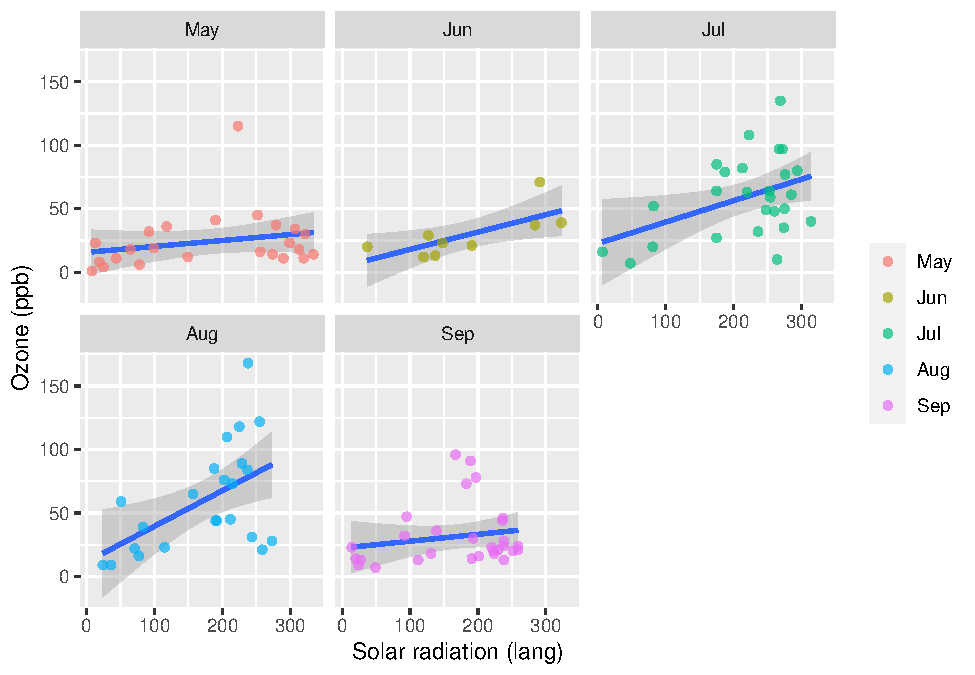
\includegraphics[width=1\linewidth,]{simple_template_files/figure-latex/plot-demo-1} \caption{Ozon concentraties geplot tegen zonlicht intensiteit, vergeleken over verschillende maanden. Lineaire modellen (blauwe lijnen) en confidence intervals (grijze gebieden) zijn hieraan toegevoegd.}\label{fig:plot-demo}
\end{figure}

Geef tabellen bovenaan een titel en bijschrift die de inhoud beschrijft en onderaan voetnoten die kolomnamen of specifieke waardes verklaren.

Deze sectie bevat tussen de 600-1200 woorden.

\hypertarget{discussie-en-conclusies}{%
\section{Discussie en Conclusies}\label{discussie-en-conclusies}}

Formuleer je conclusie door eerst in te zoomen op je eigen data en daarna uit te zoomen. Zoom in door je resultaten samen te vatten. Zoom uit om de waarde van je werk te beoordelen, door je bijvoorbeeld de volgende vragen te stellen:

\begin{itemize}
\tightlist
\item
  Kunnen mijn resultaten gebruikt worden in het werkveld?
\item
  Wat betekenen ze voor het werkveld?
\item
  Zijn mijn data betrouwbaar?
\end{itemize}

Bespreek de resultaten zodanig dat je ze ter discussie stelt, wees kritisch. Vergelijk je resultaten met de literatuur of eerder ontwikkelde data. Geef aanbevelingen voor een vervolg en staaf je aanbevelingen door de impact op wetenschappelijk of maatschappelijk vlak te beschrijven.

Kom ten slotte altijd terug op de doelstelling (en hypothesen).

Deze sectie bevat tussen de 400-800 woorden.

\hypertarget{online-bijlagen}{%
\section{Online bijlagen}\label{online-bijlagen}}

Vaak zijn online bijlagen vele malen groter dan het eigenlijke artikel. Wees nooit bang om te veel aan bijlagen aan te bieden. Je kan hierbij denken aan

\begin{itemize}
\tightlist
\item
  de ruwe data
\item
  de code voor dataverwerking
\item
  de code voor analyse
\item
  aanvullende figuren en tabellen
\end{itemize}

Natuurlijk is een git(hub) repo daar de beste plek voor!
Zorg ervoor de je repo logisch is ingericht met goede Readme document(en).
Ook de code zelf is waar nodig natuurlijk goed gedocumenteerd.

\hypertarget{wordcount}{%
\subsection{Wordcount}\label{wordcount}}

Voeg aan het eind een woord-telling in:

\begin{tabular}{l|l|l}
\hline
Method & koRpus & stringi\\
\hline
Word count & 1199 & 1198\\
\hline
Character count & 7741 & 7730\\
\hline
Sentence count & 97 & Not available\\
\hline
Reading time & 6 minutes & 6 minutes\\
\hline
\end{tabular}

\hypertarget{referenties}{%
\section{Referenties}\label{referenties}}

Een lijst van referenties wordt hier automagisch toegevoegd.

\hypertarget{refs}{}
\begin{CSLReferences}{1}{0}
\leavevmode\vadjust pre{\hypertarget{ref-xie2013ddrk}{}}%
Xie, Yihui. 2013. \emph{Dynamic Documents with R and knitr}. Boca Raton, FL: CRC Press.

\end{CSLReferences}

\end{document}
